\documentclass[
  10pt,
  a4paper,
  twocolumn,
]{article}

\usepackage{minted}
\usemintedstyle{bw}
\usepackage{caption}

\usepackage{tikz}
\usetikzlibrary{
  arrows.meta,
  positioning
}
\tikzset{
  every node/.style={draw, align=center, rounded corners},
  -{Stealth[scale=1.5]},
}

\usepackage[cm]{fullpage}

\usepackage{graphicx}
\usepackage{hyperref}

\usepackage[
	backend=biber
]{biblatex}
\bibliography{references}

\def\mytitle{Puddle: Reliable, High-Level Programming of Microfluidic Devices}
\def\myauthors{Max Willsey, Luis Ceze, ???}

\hypersetup{
  pdftitle = {\mytitle},
  pdfauthor = {\myauthors}
}

\title{\mytitle}
\author{\myauthors
\\ \small Paul G. Allen School for Computer Science and Engineering
\\ \small University of Washington}
\date{}

\begin{document}

\maketitle

Lab automation technology automatically manipulates small chemical or biological samples to save time and reagents.
While promising, these lab-on-a-chip devices are error-prone and difficult to program.
We propose a runtime system that automates error handling and resource management to provide a system-call-ish interface.
Abstracting away low-level details will make it possible to write high-level programs to automate a variety of lab protocols.

Our talk will begin by presenting the broad applications of lab automation technology.
We will describe the hardware and the challenges of programming it with existing techniques.
We will present our prototype system, explaining how it provides a higher-level programming model.
Finally, we will touch on some future work that these abstractions will enable, including connections to type systems and verification, approximate computing, and molecular computing systems.

\section*{Droplet-based Microfluidics}

While there are several kinds of lab automation devices,
droplet-based microfluidic (DMF) technology is especially promising because of its flexibility.
DMF devices manipulate individual droplets of liquids on a grid of electrodes (\autoref{fig:board}).
Activating electrodes in certain patterns can move, mix, or split droplets anywhere on the chip.

Other microfluidic technologies rely on a fixed network of channels, but DMF
devices are more flexible: think of fixed-function ASICs compared to a CPU.
Unfortunately, the tooling surrounding DMF technology offers little programming abstraction,
and the hardware itself suffers from high failure rates \cite{dmf-review}.

The ``assembly language'' that controls DMF devices is little more than controlling individual electrodes.
For example, the commands to move a droplet from cell (1,3) to cell (2,5) would be something like the following:

\begin{verbatim}
activate(1,3); activate(1,4);
activate(1,5); activate(2,5);
\end{verbatim}

Locations on the chip are referred to explicitly, and there's no notion in the program of the identity, properties, or even the existence of the droplets!
This, of course, is no way to write a program whose primary concern is manipulating droplets.

Existing work uses place-and-route techniques from VLSI to abstract away specific locations.
In this model, the program is DAG that encodes the dependencies of the operations.
\autoref{fig:dag} shows a pseudo-code snippet along with the corresponding DAG.
Tools can take such a DAG and automatically determine when and where to execute each operation \cite{grissom2015open}.
The tool then plans routes for every droplet so that they don't collide on the way.
Importantly, this is all done \emph{ahead of time}.
We don't have to waste computation at runtime creating an execution plan.
Also, we can statically determine if execution a given program on a given chip is possible.

On the other hand, static place-and-route techniques cannot offer error correction or data-dependent control flow.
For example, if the controller attempts to move a droplet but cannot, a static execution plan will just continue, and the plan's model of chip will fall out-of-sync with reality.
If a program branches on the value of a sensor reading, static execution planning gets more complicated.
While simple conditionals can be handled by ``compiling'' basic blocks, loops and procedures are still out of reach, as there's no ``stack'' on which to push an unknown amount frames.

\begin{figure}
  \hfill
  \begin{minipage}{0.45\linewidth}
    \begin{minted}[fontsize=\small]{python}
a = input(substance_A)
b = input(substance_B)
# mix in 2:1 ratio
ab = mix(a, b, 2)

heat(ab)
    \end{minted}
  \end{minipage}
  \hfill
  \begin{minipage}{0.45\linewidth}
    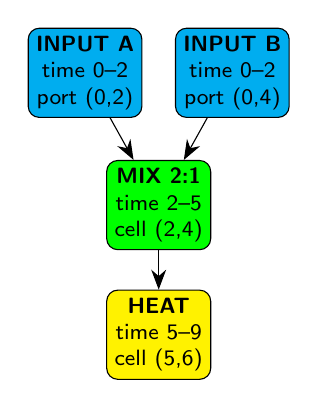
\begin{tikzpicture}
      \footnotesize \sf
      \node[draw=none] (mid) {};
      \node (A) [left = 1mm of mid, fill=cyan] {
        \textbf{INPUT A} \\
        time 0--2 \\
        port (0,2)
      };
      \node (B) [right = 1mm of mid, fill=cyan] {
        \textbf{INPUT B} \\
        time 0--2 \\
        port (0,4)
      };
      \node (mix) [below = 10mm of mid, fill=green] {
        \textbf{MIX 2:1} \\
        time 2--5 \\
        cell (2,4)
      };
      \node (heat) [below = 5mm of mix, fill=yellow] {
        \textbf{HEAT} \\
        time 5--9 \\
        cell (5,6)
      };

      \draw (A) -- (mix);
      \draw (B) -- (mix);
      \draw (mix) -- (heat);
    \end{tikzpicture}
  \end{minipage}

  \caption{
    Fluidic program and the corresponding DAG where the operations have been
    scheduled and placed.
  }
\label{fig:dag}
\end{figure}

\vfill

\renewcommand*{\bibfont}{\footnotesize}
\printbibliography[heading=none]

\end{document}